\documentclass[a4paper,11pt]{jsarticle}

% パッケージ
\usepackage[dvipdfmx]{hyperref}
\usepackage{pxjahyper}
\usepackage[dvipdfmx]{graphicx}
\usepackage{ascmac}
\usepackage{fancybox}
\usepackage{listings}
\usepackage{plistings}
\usepackage{multirow}
\usepackage[subrefformat=parens]{subcaption}
\usepackage{color}
\usepackage{here}
\usepackage{amsmath,amsfonts}
\usepackage[utf8]{inputenc}
\usepackage{bm}
\usepackage{siunitx}
\usepackage{url}
\usepackage{longtable}
% ページの周りの余白
\usepackage[top=25truemm,bottom=25truemm,left=30truemm,right=30truemm]{geometry}

% URLの設定
\Urlmuskip=0mu  plus 10mu

% 色の定義
\definecolor{OliveGreen}{rgb}{0.0,0.6,0.0}
\definecolor{Magenta}{cmyk}{0, 1, 0, 0}
\definecolor{colFunc}{rgb}{1,0.07,0.54}
\definecolor{CadetBlue}{cmyk}{0.62,0.57,0.23,0}
\definecolor{Brown}{cmyk}{0,0.81,1,0.60}
\definecolor{colID}{rgb}{0.63,0.44,0}


\lstset{
  basicstyle={\ttfamily},
  identifierstyle={\small},
  commentstyle={\smallitshape},
  keywordstyle={\small\bfseries},
  ndkeywordstyle={\small},
  stringstyle={\small\ttfamily},
  frame={tb},
  breaklines=true,
  columns=[l]{fullflexible},
  numbers=left,
  xrightmargin=0zw,
  xleftmargin=3zw,
  numberstyle={\scriptsize},
  stepnumber=1,
  numbersep=1zw,
  lineskip=-0.5ex
}

\renewcommand{\lstlistingname}{Code}

% リンクの設定
\hypersetup{
  setpagesize=false,
  bookmarksnumbered=true,
  bookmarksopen=true,
  colorlinks=true,
  linkcolor=blue,
  citecolor=red,
}

\begin{document}

%\title{}
%\author{}
%\date{\today}
%\maketitle


\section{目的}
本実験は,抵抗$R$とコンデンサ$C$の2つの素子で構成されるフィルタ回路の周波数応答を調べ,
フィルタ回路についての理解を深めることを目的とする.

\section{概要}
\subsection{フィルタ回路とは}
インダクタのインピーダンスは周波数に比例し,コンデンサのインピーダンスは周波数に反比例する.
これらの特性を利用することで,入力信号の特定の周波数に対して「通過」もしくは「遮断」することができる.
これらの現象は「フィルタ」と呼ばれ,これらの動作を行う回路をフィルタ回路~\cite{text}~\cite{filtar}と呼ぶ.

\subsection{フィルタの種類}
以下の図\ref{Ex_filtar}にフィルタの種類とその特徴を示す.
\begin{figure}[H]
  \begin{minipage}{0.48\textwidth}
    \begin{center}
      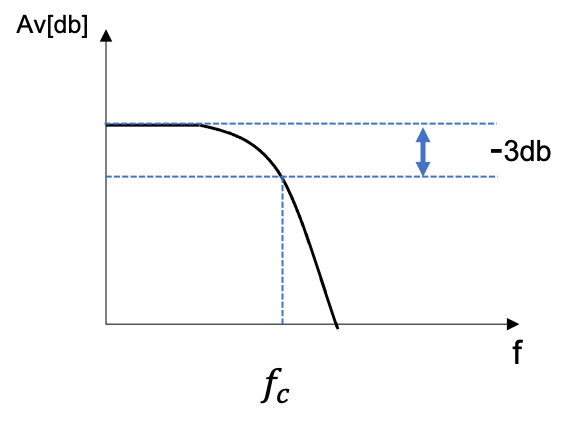
\includegraphics[clip,width=7.5cm]{picture/E_LPF.png}
    \end{center}
    \subcaption{ローパスフィルタ}
    \label{Ex_LPF}
  \end{minipage}
  \begin{minipage}{0.48\textwidth}
    \begin{center}
      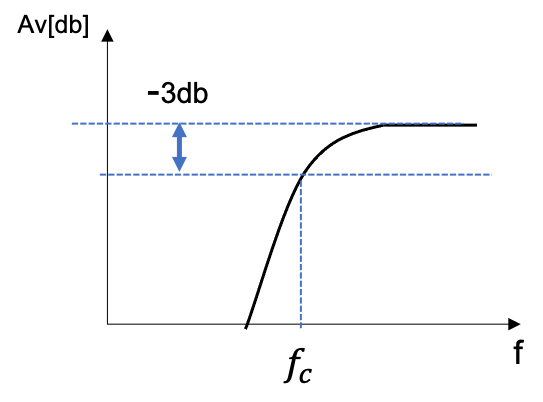
\includegraphics[clip,width=7.5cm]{picture/E_HPF.png}
    \end{center}
    \subcaption{ハイパスフィルタ}
    \label{Ex_HPF}
  \end{minipage} \\
  \begin{minipage}{0.48\textwidth}
    \begin{center}
      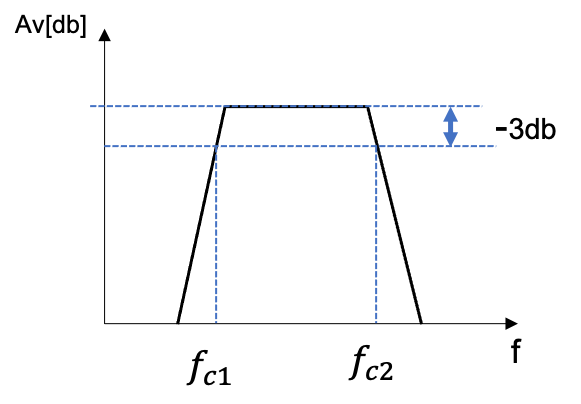
\includegraphics[clip,width=7.5cm]{picture/E_BPF.png}
    \end{center}
    \subcaption{バンドパスフィルタ}
    \label{Ex_BPF}
  \end{minipage}
  \begin{minipage}{0.48\textwidth}
    \begin{center}
      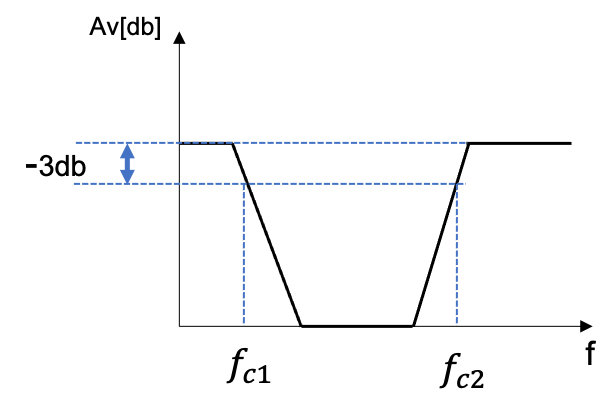
\includegraphics[clip,width=7.5cm]{picture/E_BSF.png}
    \end{center}
    \subcaption{バンドストップフィルタ}
    \label{Ex_BSF}
  \end{minipage}
  \caption{フィルタの種類}
  \label{Ex_filtar}
\end{figure}
\begin{enumerate}
  \item ローパスフィルタ(低域通過型フィルタ,LPF)(図\ref{Ex_LPF})
        ある周波数$f_c$より低い周波数帯域の信号のみを通すフィルタ.
  \item ハイパスフィルタ(高域通過型フィルタ,HPF)(図\ref{Ex_HPF})
        ある周波数$f_c$より高い周波数帯域の信号のみを通すフィルタ.
  \item バンドパスフィルタ(帯域通過型フィルタ,BPF)(図\ref{Ex_BPF})
        カットオフ周波数$f_{c1},f_{c2}$を持ち,それらの間の周波数帯域の信号のみ
        を通すフィルタ.中心周波数$f_0$付近の周波数を取り出すための目的にも利用されることもある.
  \item バンドストップフィルタ(帯域阻止型フィルタ,BSP)(図\ref{sub@Ex_BSF})
        バンドパスフィルタとは反対に,カットオフ周波数$f_{c1},f_{c2}$に挟まれた周波数帯域の
        信号を阻止し,それ以外の信号を通すフィルタ.バンドリジェクションフィルタとも呼ばれる.
\end{enumerate}

\subsection{RCローパスフィルタ}
以下の図\ref{RC_LPF}にRC型ローパスフィルタの回路を示す.
\begin{figure}[H]
  \centering
  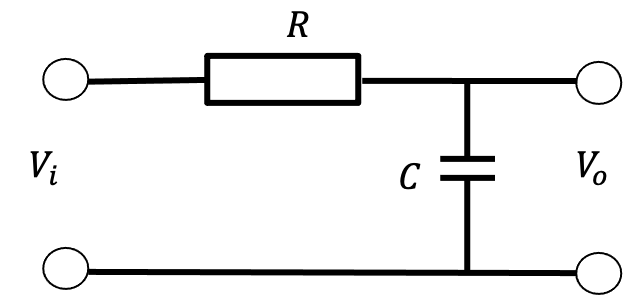
\includegraphics[width=0.3\linewidth]{picture/RC_LPF.png}
  \caption{RC型ローパスフィルタ}
  \label{RC_LPF}
\end{figure}
この回路における$V_i$と$V_o$の関係を
分圧則を用いて考えると,以下の式\ref{F:Vo_Vi_LPF}のように表すことができる.
\begin{equation}
  V_o = \frac{\frac{1}{j\omega C}}{R+\frac{1}{j\omega C}}V_i = \frac{1}{1+j\omega RC}V_i \label{F:Vo_Vi_LPF}
\end{equation}
また,このときの$V_i$と$V_o$の比の絶対値(ゲイン)は以下の式\ref{F:G_LPF}のようになる.
\begin{equation}
  G = \left|\frac{V_o}{V_i}\right| = \frac{1}{\sqrt{1 + \omega^2R^2C^2}} \label{F:G_LPF}
\end{equation}
ゲインGを用いると,電圧利得を以下の式\ref{F:A_LPF}で表すことができる.
\begin{equation}
  A = 20\log{G} [\si{\deci \bel}]\label{F:A_LPF}
\end{equation}
式\ref{F:A_LPF}において,$A=-3\si{\deci \bel}$となる周波数はカットオフ周波数と言われ,$f_c$で表される.
RC型ローパスフィルタのカットオフ周波数は以下の式\ref{F:fc_LPF}となる.
\begin{equation}
  f_c = \frac{1}{2\pi RC} \label{F:fc_LPF}
\end{equation}

\subsection{RCハイパスフィルタ}
以下の図\ref{RC_HPF}にRC型ハイパスフィルタの回路を示す.
\begin{figure}[H]
  \centering
  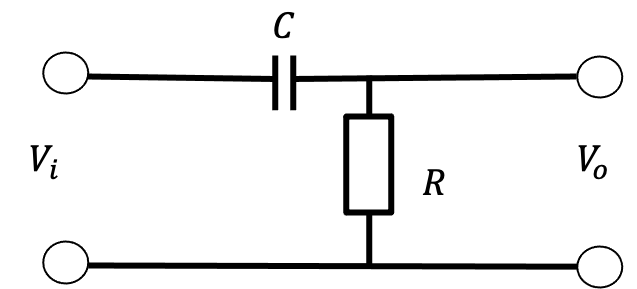
\includegraphics[width=0.3\linewidth]{picture/RC_HPF.png}
  \caption{RC型ハイパスフィルタ}
  \label{RC_HPF}
\end{figure}
この回路における$V_i$と$V_o$の関係を
分圧則を用いて考えると,以下の式\ref{F:Vo_Vi_HPF}のように表すことができる.
\begin{equation}
  V_o = \frac{R}{R+\frac{1}{j\omega C}}V_i = \frac{j\omega RC}{1+j\omega RC}V_i \label{F:Vo_Vi_HPF}
\end{equation}
また,このときの$V_i$と$V_o$の比の絶対値(ゲイン)は以下の式\ref{F:G_HPF}のようになる.
\begin{equation}
  G = \left|\frac{V_o}{V_i}\right| = \frac{\omega RC}{\sqrt{1 + \omega^2R^2C^2}} \label{F:G_HPF}
\end{equation}
ゲインGを用いると,電圧利得を以下の式\ref{F:A_HPF}で表すことができる.
\begin{equation}
  A = 20\log{G} [\si{\deci \bel}]\label{F:A_HPF}
\end{equation}
式\ref{F:A_HPF}において,$A=-3\si{\deci \bel}$となる周波数はカットオフ周波数と言われ,$f_c$で表される.
RC型ローパスフィルタのカットオフ周波数は以下の式\ref{F:fc_HPF}となる.
\begin{equation}
  f_c = \frac{1}{2\pi RC} \label{F:fc_HPF}
\end{equation}

\section{実験環境}
以下の表\ref{T:location}に使用した実験器具を示す.
\begin{table}[H]
  \begin{center}
    \caption{使用した実験器具}
    \begin{tabular}{|c|c|} \hline
      ファンクションジェネレータ & RIGOL DG1022 No.23                 \\ \hline
      オシロスコープ             & Agilent Technologies DSO1024A No.2 \\ \hline
      定抵抗                     & $996.8\si{\ohm}$                   \\ \hline
      コンデンサ                 & $0.476\si{\mu F}$                  \\ \hline
      ブレッドボード             &                                    \\ \hline
      配線ケーブル               &                                    \\ \hline
    \end{tabular}
    \label{T:location}
  \end{center}
\end{table}

\section{実験方法}
本実験は実験資料~\cite{text}に準じて行う.以下にローパスフィルタとハイパスフィルタそれぞれの実験手順
について示す.
\subsection{ローパスフィルタの周波数特性測定}
\begin{enumerate}
  \item 定抵抗とコンデンサを使用し,図\ref{RC_LPF}の回路を作成する.
  \item ファンクションジェネレータで振幅を$5\si{\volt}$に調節し,フィルタ回路の入力に接続する.
  \item オシロスコープのCH1で入力信号を測定し,CH2で出力信号を測定する.
  \item 入力信号の周波数を任意の値に変更しながら,CH1とCH2の信号を同時に観測し,振幅を計算する.
  \item 実行結果をもとに,電圧利得($\si{\deci \bel}$)を計算しグラフ化する.
\end{enumerate}
\subsection{ハイパスフィルタの周波数特性測定}
\begin{enumerate}
  \item 定抵抗とコンデンサを使用し,図\ref{RC_HPF}の回路を作成する.
  \item ファンクションジェネレータで振幅を$5\si{\volt}$に調節し,フィルタ回路の入力に接続する.
  \item オシロスコープのCH1で入力信号を測定し,CH2で出力信号を測定する.
  \item 入力信号の周波数を任意の値に変更しながら,CH1とCH2の信号を同時に観測し,振幅を計算する.
  \item 実行結果をもとに,電圧利得($\si{\deci \bel}$)を計算しグラフ化する.
\end{enumerate}

\section{実験結果}
\subsection{ローパスフィルタの周波数特性測定}
以下の表\ref{T:LPF_result}と図\ref{G:LPF_result}にローパスフィルタ回路における測定結果を示す.
\begin{center}
  \begin{longtable}{|c|c|c|c|c|c|c|}
    \caption{ローパスフィルタ回路の測定結果}
    \label{T:LPF_result}
    \endhead
    \hline
    Freq[$\si{\hertz}$] & $V_{out}$ & $V_{in}$ & G(測定値)   & db           & G(理論値)   & db(理論値)   \\ \hline
    10                  & 9         & 10.6     & 0.849056604 & -1.421267117 & 0.971715923 & -0.249213616 \\ \hline
    15                  & 9.3       & 10.4     & 0.894230769 & -0.971007815 & 0.958445116 & -0.368655026 \\ \hline
    20                  & 10        & 10.2     & 0.980392157 & -0.172003435 & 0.94570359  & -0.484899244 \\ \hline
    30                  & 9.7       & 10.2     & 0.950980392 & -0.43656875  & 0.921674322 & -0.708450242 \\ \hline
    50                  & 10.4      & 10.4     & 1           & 0            & 0.878644489 & -1.123736209 \\ \hline
    60                  & 9.8       & 10.4     & 0.942307692 & -0.516145272 & 0.859272816 & -1.317378549 \\ \hline
    70                  & 10.6      & 10.4     & 1.019230769 & 0.165450519  & 0.841128397 & -1.50275409  \\ \hline
    80                  & 10.4      & 10.4     & 1           & 0            & 0.824086893 & -1.680539866 \\ \hline
    90                  & 10.4      & 10.4     & 1           & 0            & 0.808040912 & -1.851332998 \\ \hline
    100                 & 10.6      & 10.2     & 1.039215686 & 0.33411387   & 0.792897156 & -2.015662802 \\ \hline
    150                 & 9.8       & 10.2     & 0.960784314 & -0.347481921 & 0.728177601 & -2.755253683 \\ \hline
    200                 & 9         & 10.2     & 0.882352941 & -1.087153246 & 0.677093102 & -3.387032219 \\ \hline
    250                 & 8.2       & 10.2     & 0.803921569 & -1.895726388 & 0.635442967 & -3.938468458 \\ \hline
    300                 & 7.8       & 10.2     & 0.764705882 & -2.330111381 & 0.600640332 & -4.427710182 \\ \hline
    350                 & 7.4       & 10.2     & 0.725490196 & -2.787369041 & 0.570993573 & -4.867375597 \\ \hline
    400                 & 6.8       & 10.2     & 0.666666667 & -3.521825181 & 0.545343693 & -5.266594096 \\ \hline
    450                 & 6.4       & 10.2     & 0.62745098  & -4.048403956 & 0.522866444 & -5.632184578 \\ \hline
    500                 & 6         & 10.2     & 0.588235294 & -4.608978428 & 0.502957466 & -5.969374814 \\ \hline
    550                 & 5.4       & 10.2     & 0.529411765 & -5.524128239 & 0.485162195 & -6.282260957 \\ \hline
    600                 & 5.2       & 10.2     & 0.509803922 & -5.851936563 & 0.469131275 & -6.574112275 \\ \hline
    650                 & 4.8       & 10       & 0.48        & -6.375175252 & 0.454591187 & -6.847579756 \\ \hline
    700                 & 4.6       & 10       & 0.46        & -6.744843366 & 0.441324319 & -7.104842805 \\ \hline
    750                 & 4.6       & 10       & 0.46        & -6.744843366 & 0.429155079 & -7.347714869 \\ \hline
    800                 & 4.2       & 10       & 0.42        & -7.535014192 & 0.417940009 & -7.57772104  \\ \hline
    850                 & 4         & 10       & 0.4         & -7.958800173 & 0.407560601 & -7.796156128 \\ \hline
    900                 & 4         & 10       & 0.4         & -7.958800173 & 0.397917976 & -8.004128811 \\ \hline
    1000                & 3.6       & 10       & 0.36        & -8.873949985 & 0.380522733 & -8.392387857 \\ \hline
    2000                & 2.2       & 10       & 0.22        & -13.15154638 & 0.279373335 & -11.07630095 \\ \hline
    3000                & 1         & 10       & 0.1         & -20          & 0.231133832 & -12.72272959 \\ \hline
    4000                & 0.82      & 10       & 0.082       & -21.72372295 & 0.201518002 & -13.91372302 \\ \hline
    5000                & 0.66      & 10.2     & 0.064705882 & -23.78112472 & 0.180979628 & -14.84740616 \\ \hline
    6000                & 0.56      & 10.2     & 0.054901961 & -25.2082429  & 0.165663835 & -15.61544581 \\ \hline
    7000                & 0.48      & 10.2     & 0.047058824 & -26.54717869 & 0.153676459 & -16.2678531  \\ \hline
    8000                & 0.42      & 10.2     & 0.041176471 & -27.70701763 & 0.143963816 & -16.83493299 \\ \hline
    9000                & 0.38      & 10.2     & 0.037254902 & -28.5763315  & 0.135886941 & -17.33644556 \\ \hline
  \end{longtable}
\end{center}

また,以下の図\ref{P:Scope_LPF}に実験中に取得したオシロスコープの波形を示す.
\begin{figure}[H]
  \begin{center}
    \begin{minipage}{0.48\textwidth}
      \begin{center}
        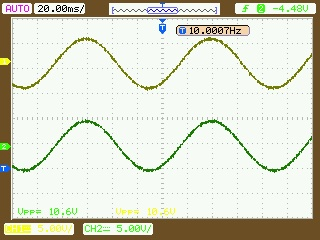
\includegraphics[clip,width=6cm]{picture/LPF/10.jpeg}
      \end{center}
      \subcaption{$10\si{\hertz}$のとき}
      \label{P:LPF_10}
    \end{minipage}
    \begin{minipage}{0.48\textwidth}
      \begin{center}
        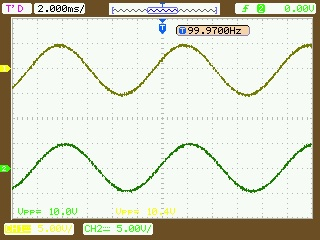
\includegraphics[clip,width=6cm]{picture/LPF/100.jpeg}
      \end{center}
      \subcaption{$100\si{\hertz}$のとき}
      \label{P:LPF_100}
    \end{minipage} \\
    \begin{minipage}{0.48\textwidth}
      \begin{center}
        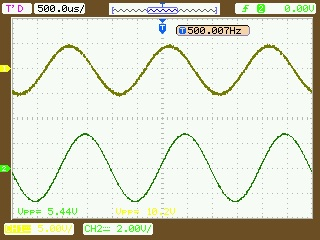
\includegraphics[clip,width=6cm]{picture/LPF/500.jpeg}
      \end{center}
      \subcaption{$500\si{\hertz}$のとき}
      \label{P:LPF_500}
    \end{minipage}
    \begin{minipage}{0.48\textwidth}
      \begin{center}
        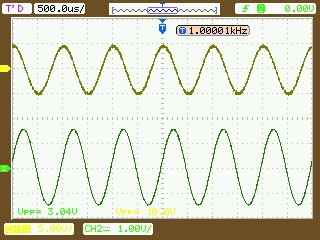
\includegraphics[clip,width=6cm]{picture/LPF/1000.jpeg}
      \end{center}
      \subcaption{$1000\si{\hertz}$のとき}
      \label{P:LPF_1000}
    \end{minipage} \\
    \begin{minipage}{0.48\textwidth}
      \begin{center}
        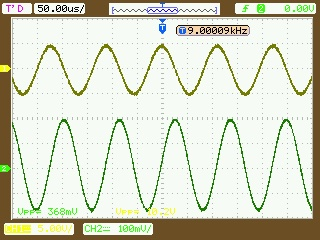
\includegraphics[clip,width=6cm]{picture/LPF/9000.jpeg}
      \end{center}
      \subcaption{$9000\si{\hertz}$のとき}
      \label{P:LPF_9000}
    \end{minipage}
    \caption{LPF回路におけるオシロスコープの出力}
    \label{P:Scope_LPF}
  \end{center}
\end{figure}

\begin{figure}[H]
  \centering
  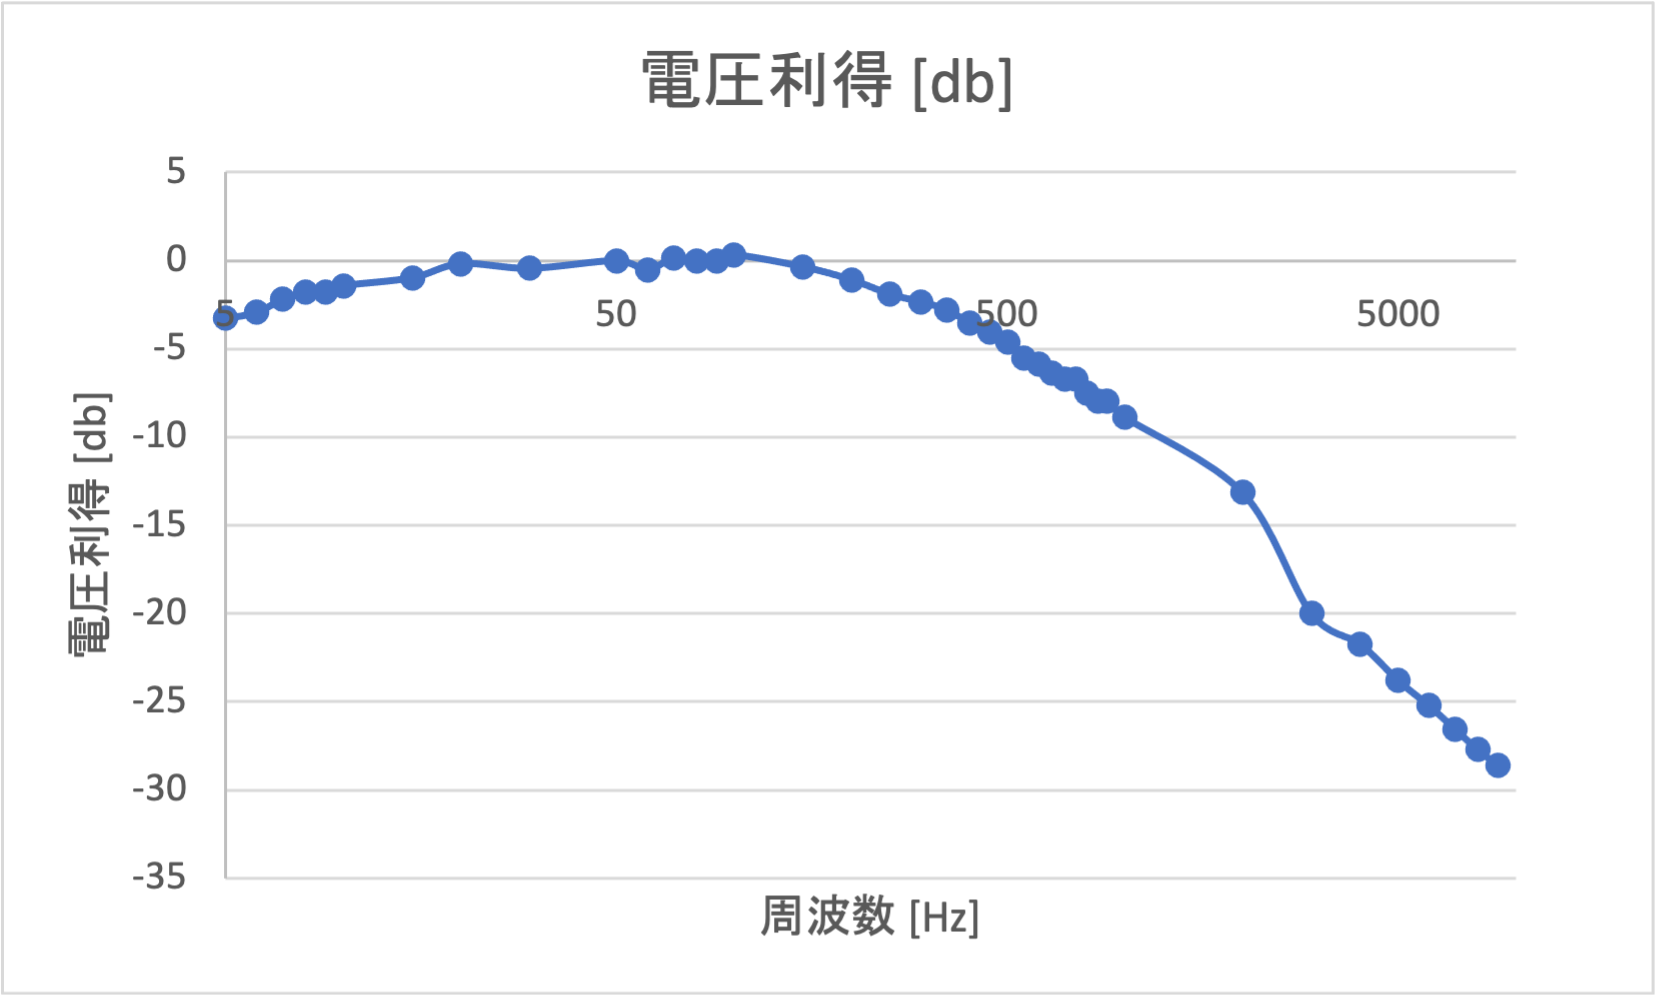
\includegraphics[width=0.8\linewidth]{picture/G_LPF_db.png}
  \caption{ローパスフィルタ回路の測定結果}
  \label{G:LPF_result}
\end{figure}
以上のデータからもわかるように,周波数が低い領域では$V_{in}とV_{out}$はほとんど変わりがなく,信号が
通過していて,周波数が高い領域では$V_{out}$がとても低くなり,ほとんどの信号を阻止していることがわかる.
図\ref{P:LPF_10}を見ると,入力信号(黄)と出力信号(緑)は振幅は変化がないが,図\ref{P:LPF_9000}では
振幅に大きな違いが見られ,RC型ローパスフィルタが正常に動作したことがわかる.
\subsection{ハイパスフィルタの周波数特性測定}
\begin{center}
  \begin{longtable}{|c|c|c|c|c|c|c|}
    \caption{ハイパスフィルタ回路の測定結果}
    \label{T:HPF_result}
    \endhead
    \hline
    Freq[$\si{\hertz}$] & $V_{out}$ & $V_{in}$ & G(測定値)   & db(測定値)   & G(理論値)   & db(理論値)   \\ \hline
    10                  & 0.288     & 10.4     & 0.027692308 & -31.15281703 & 0.029104358 & -30.72083963 \\ \hline
    20                  & 0.6       & 10.6     & 0.056603774 & -24.9430923  & 0.057391429 & -24.82305918 \\ \hline
    30                  & 0.88      & 10.4     & 0.084615385 & -21.45101334 & 0.084911445 & -21.42067541 \\ \hline
    40                  & 1.17      & 10.4     & 0.1125      & -18.97694955 & 0.111710181 & -19.03814489 \\ \hline
    50                  & 1.47      & 10.6     & 0.138679245 & -17.15977061 & 0.137829469 & -17.21315837 \\ \hline
    60                  & 1.84      & 10.4     & 0.176923077 & -15.04431033 & 0.163307626 & -15.73987071 \\ \hline
    70                  & 2.16      & 10.6     & 0.203773585 & -13.81704228 & 0.188179837 & -14.50853825 \\ \hline
    80                  & 2.4       & 10.4     & 0.230769231 & -12.73644195 & 0.212478481 & -13.45370094 \\ \hline
    90                  & 2.72      & 10.6     & 0.256603774 & -11.81473922 & 0.23623342  & -12.53317325 \\ \hline
    100                 & 2.96      & 10.4     & 0.284615385 & -10.91483256 & 0.259472249 & -11.71818168 \\ \hline
    150                 & 4.3       & 10.6     & 0.405660377 & -7.836748194 & 0.368757747 & -8.665176953 \\ \hline
    200                 & 5.2       & 10.2     & 0.509803922 & -5.851936563 & 0.468300457 & -6.589508363 \\ \hline
    250                 & 6         & 10.2     & 0.588235294 & -4.608978428 & 0.559962036 & -5.036828327 \\ \hline
    300                 & 6.6       & 10.2     & 0.647058824 & -3.781124724 & 0.645113747 & -3.807274062 \\ \hline
    350                 & 7.1       & 10.2     & 0.696078431 & -3.146836461 & 0.724794208 & -2.795705713 \\ \hline
    400                 & 7.5       & 10       & 0.75        & -2.498774732 & 0.799808668 & -1.940277866 \\ \hline
    450                 & 7.8       & 10.2     & 0.764705882 & -2.330111381 & 0.870793959 & -1.201691845 \\ \hline
    500                 & 8         & 10.2     & 0.784313725 & -2.110203695 & 0.938262389 & -0.553513845 \\ \hline
    550                 & 8.3       & 10.2     & 0.81372549  & -1.790441588 & 1.002632248 & 0.022833374  \\ \hline
    600                 & 8.4       & 10.2     & 0.823529412 & -1.686417714 & 1.064249531 & 0.540869352  \\ \hline
    650                 & 8.5       & 10       & 0.85        & -1.411621486 & 1.123403747 & 1.010717359  \\ \hline
    700                 & 8.7       & 10       & 0.87        & -1.209614948 & 1.180339623 & 1.440139729  \\ \hline
    750                 & 8.8       & 10       & 0.88        & -1.110346557 & 1.235265945 & 1.835209368  \\ \hline
    800                 & 8.8       & 10       & 0.88        & -1.110346557 & 1.288362301 & 2.20076017   \\ \hline
    850                 & 8.8       & 10.2     & 0.862745098 & -1.282349992 & 1.339784333 & 2.540697898  \\ \hline
    900                 & 8.9       & 10       & 0.89        & -1.012199867 & 1.389667839 & 2.858220137  \\ \hline
    950                 & 9         & 10.2     & 0.882352941 & -1.087153246 & 1.438132048 & 3.155975287  \\ \hline
    1000                & 9         & 10       & 0.9         & -0.915149811 & 1.485282231 & 3.436179711  \\ \hline
    1500                & 9.3       & 10.2     & 0.911764706 & -0.802344464 & 1.901004925 & 5.579664838  \\ \hline
    2000                & 9.4       & 10.2     & 0.921568627 & -0.709446363 & 2.247441154 & 7.033766582  \\ \hline
    2500                & 9.4       & 10       & 0.94        & -0.537442928 & 2.549908907 & 8.130493319  \\ \hline
    3000                & 9.4       & 10.2     & 0.921568627 & -0.709446363 & 2.821474517 & 9.009522644  \\ \hline
    3500                & 9.4       & 10.2     & 0.921568627 & -0.709446363 & 3.069862475 & 9.742378404  \\ \hline
    4000                & 9.4       & 10       & 0.94        & -0.537442928 & 3.300066338 & 10.3704534   \\ \hline
  \end{longtable}
\end{center}

\begin{figure}[H]
  \centering
  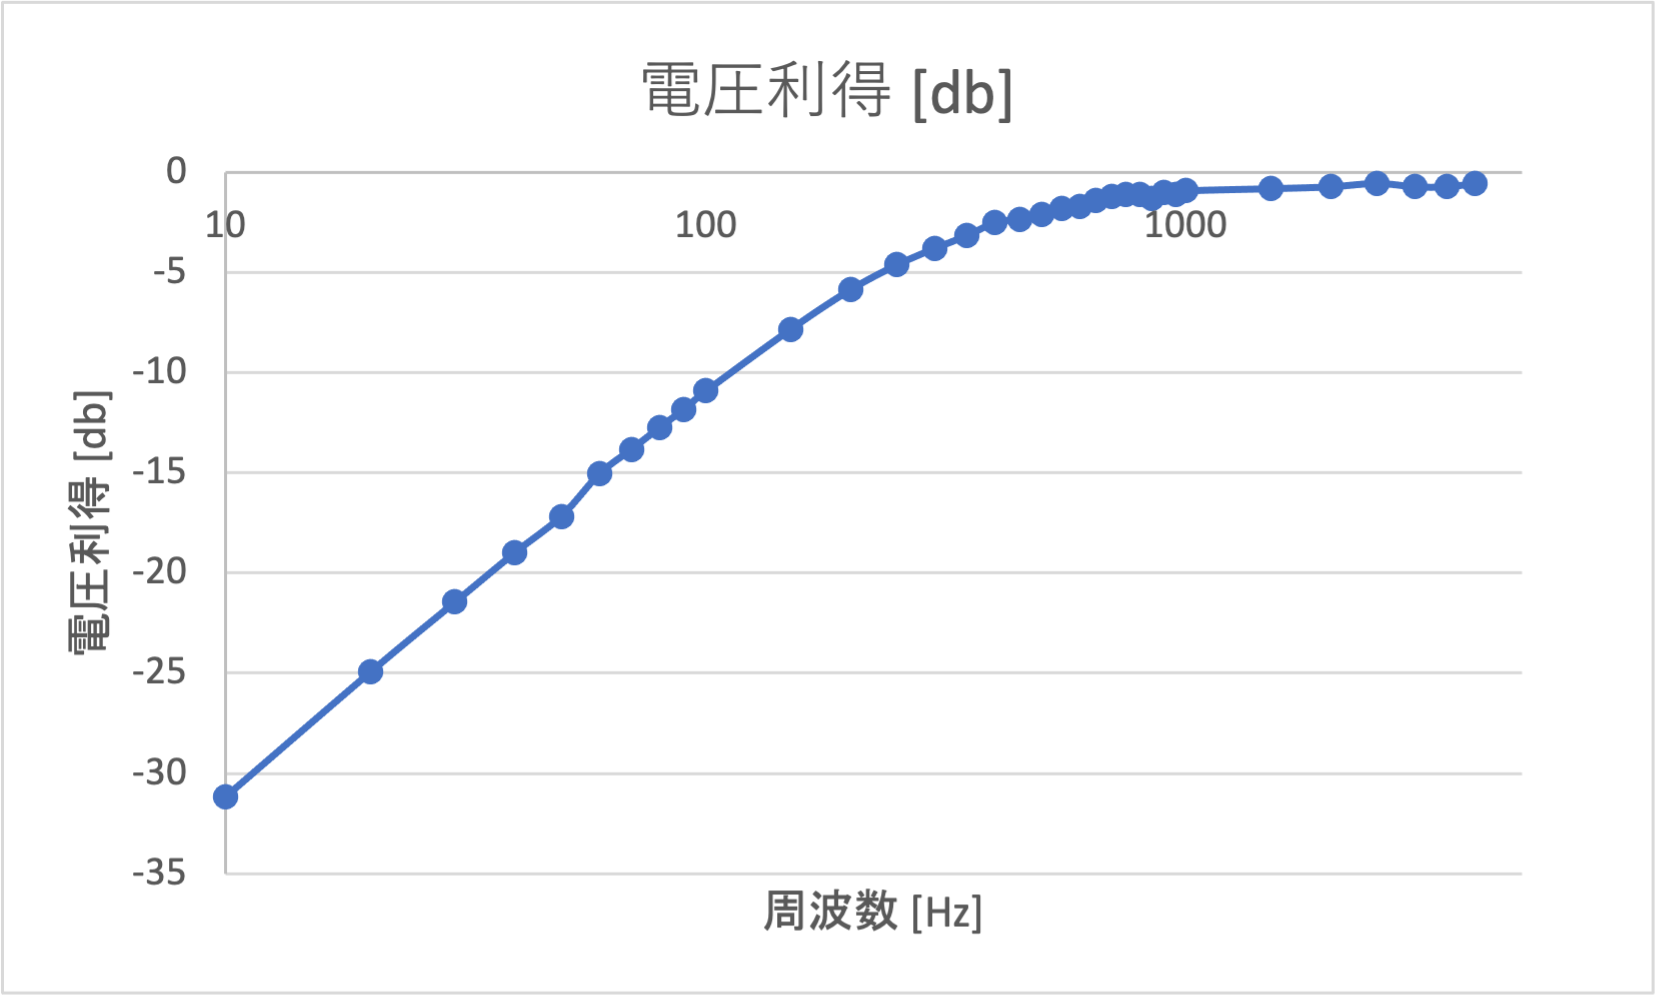
\includegraphics[width=0.8\linewidth]{picture/G_HPF_db.png}
  \caption{ハイパスフィルタ回路の測定結果}
  \label{G:HPF_result}
\end{figure}
また,以下の図\ref{P:Scope_HPF}に実験中に取得したオシロスコープの波形を示す.
\begin{figure}[H]
  \begin{center}
    \begin{minipage}{0.48\textwidth}
      \begin{center}
        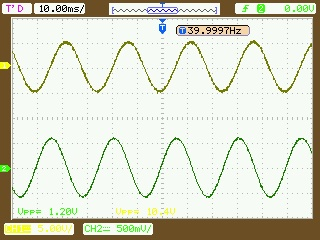
\includegraphics[clip,width=6cm]{picture/HPF/40.jpeg}
      \end{center}
      \subcaption{$40\si{\hertz}$のとき}
      \label{P:HPF_40}
    \end{minipage}
    \begin{minipage}{0.48\textwidth}
      \begin{center}
        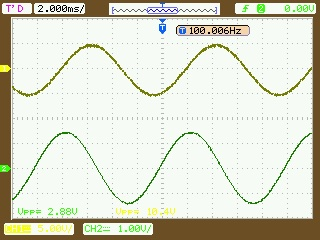
\includegraphics[clip,width=6cm]{picture/HPF/100.jpeg}
      \end{center}
      \subcaption{$100\si{\hertz}$のとき}
      \label{P:HPF_100}
    \end{minipage} \\
    \begin{minipage}{0.48\textwidth}
      \begin{center}
        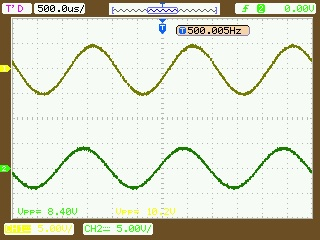
\includegraphics[clip,width=6cm]{picture/HPF/500.jpeg}
      \end{center}
      \subcaption{$500\si{\hertz}$のとき}
      \label{P:HPF_500}
    \end{minipage}
    \begin{minipage}{0.48\textwidth}
      \begin{center}
        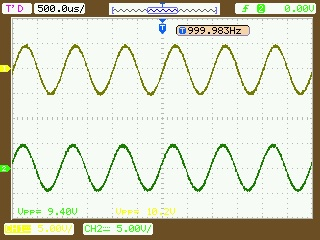
\includegraphics[clip,width=6cm]{picture/HPF/1000.jpeg}
      \end{center}
      \subcaption{$1000\si{\hertz}$のとき}
      \label{P:HPF_1000}
    \end{minipage}
    \caption{HPF回路におけるオシロスコープの出力}
    \label{P:Scope_HPF}
  \end{center}
\end{figure}
以上のデータからもわかるように,周波数が高い領域では$V_{in}とV_{out}$はほとんど変わりがなく,信号が
通過していて,周波数が低い領域では$V_{out}$がとても低くなり,ほとんどの信号を阻止していることがわかる.
図\ref{P:HPF_1000}を見ると,入力信号(黄)と出力信号(緑)は振幅は変化がないが,図\ref{P:HPF_40}では
振幅に大きな違いが見られ,RC型ハイパスフィルタが正常に動作したことがわかる.

\section{考察}
\subsection{カットオフ周波数}
本実験でのカットオフ周波数を式\ref{F:fc_LPF},\ref{F:fc_HPF}を用いて計算する.本実験で使用した
抵抗$R$とコンデンサ$C$はそれぞれ表\ref{T:location}に示した値であり多少の誤差が含まれる.
以下の式\ref{F:fc_sokutei}に測定値から求めたカットオフ周波数を示し,式\ref{F:fc_rironn}
に理論値から求めたカットオフ周波数を示す.
\begin{align}
  f_c & = \frac{1}{2\pi RC}                                       \nonumber \\
      & = \frac{1}{2\pi \times 996.8 \times 0.496 \times 10^{-6}} \nonumber \\
      & = 321.907 \ \ \ \si{\hertz} \label{F:fc_sokutei}
\end{align}
\begin{align}
  f_c & = \frac{1}{2\pi RC}                                     \nonumber \\
      & = \frac{1}{2\pi \times 1000 \times 0.47 \times 10^{-6}} \nonumber \\
      & = 338.628 \ \ \ \si{\hertz} \label{F:fc_rironn}
\end{align}
上式や,実験結果からわかるようにカットオフ周波数に理論値と異なるズレが生じた.これらは
回路に用いた素子の誤差が原因だと考えられる.

\subsection{バンドパスフィルタ回路}
バンドパスフィルタ~\cite{BPF}は図\ref{Ex_BPF}に示したような特徴をもつフィルタであり,LPFとHPF
2つを用いることで作成することができる.以下の図\ref{C:RLC_BPF}に回路例を示す.
\begin{figure}[H]
  \centering
  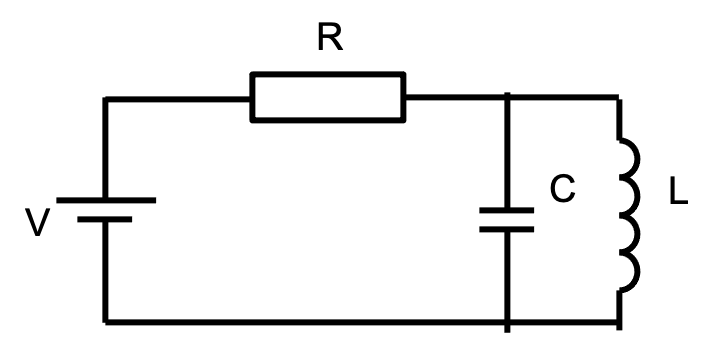
\includegraphics[width=0.3\linewidth]{picture/RLC_BPF.png}
  \caption{バンドパスフィルタの回路例}
  \label{C:RLC_BPF}
\end{figure}
この回路における共振周波数が,バンドパスフィルタの信号を一番多く通す周波数帯であり,共振周波数は以下の式\ref{f0}
で示される.
\begin{equation}
  \frac{1}{2\pi\sqrt{LC}} \label{f0}
\end{equation}

\subsection{バンドストップフィルタ回路}
バンドストップフィルタ~\cite{BEF}とは,ある範囲の信号のみを減衰させ,それ以外の信号を通すフィルタのことであり,
減衰させる周波数の範囲が狭くなったものはノッチフィルタと言われている.以下の図\ref{C:BEF}にノッチフィルタ回路の例を
示す.
\begin{figure}[H]
  \centering
  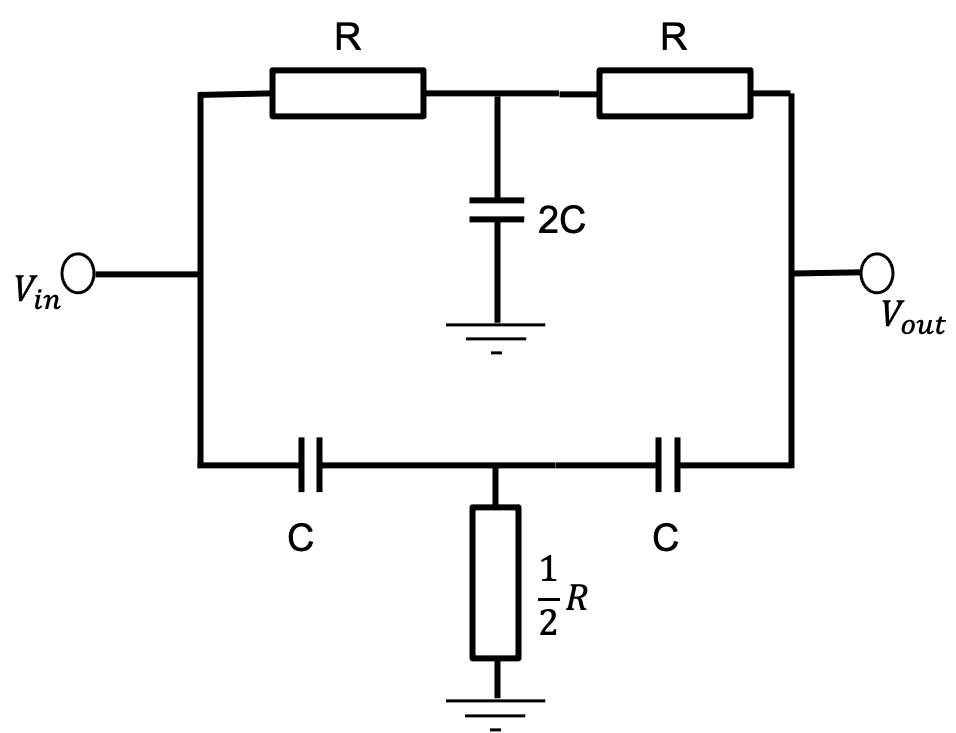
\includegraphics[width=0.3\linewidth]{picture/BEF_C.png}
  \caption{ノッチフィルタの回路例}
  \label{C:BEF}
\end{figure}
減衰させる周波数は以下の式\ref{F:BEF}で示すことができる.
\begin{equation}
  f_N = \frac{1}{2\pi CR} \label{F:BEF}
\end{equation}
\begin{thebibliography}{99}
  \bibitem{text} 制御情報システム工学科 4 年実験指導書: ''フィルタ回路'', 2020 (最終閲覧日 2021年7月1日)\\
  \bibitem{filtar} APS: ''ローパスフィルタとハイパスフィルタを学ぶ'' (最終閲覧日 2021年7月1日) \\ \url{https://www.aps-web.jp/academy/ec/539/}
  \bibitem{BPF} APS: ''バンドパスフィルタで特定の周波数範囲を扱う'' (最終閲覧日 2021年7月5日) \\ \url{https://www.aps-web.jp/academy/ec/541/}
  \bibitem{BEF} Electrical information: ''【ノッチフィルタとは】設計方法や用途について'' (最終閲覧日 2021年7月5日) \\ \url{https://detail-infomation.com/notch-filter/}
\end{thebibliography}

\end{document}